\documentclass[fleqn]{jbook}
\usepackage{physpub}
\usepackage{txfonts}

\newcommand{\pr}[1]{#1^{\,\prime}}  %プライム
\newcommand{\erf}{\mathop{\rm erf}\nolimits} %誤差関数
\newcommand{\diff}[2]{\frac{\mathrm{d} #1}{\mathrm{d} #2}}   %微分
\newcommand{\prt}[2]{\frac{\partial #1}{\partial #2}}   %偏微分
\newcommand{\prts}[3]{\frac{\partial^{#3} #1}{\partial {#2}^{#3}}}   %n回偏微分


\begin{document}

%%%%%【数学1 問題】%%%%%%%%%%%%%%%%%%%%%%%%%%%%%%%%%%%%%%%%%%%%%%%%%%%%%%%
\begin{question}{問題1}{藤野健}
\setcounter{equation}{0}

変数$x$についての2次以下の次数の多項式のなす線形空間を$V$とする。

線形写像$F:V \longrightarrow V$を以下のように定める。
\[
    \mbox{任意の}p(x) \in V \mbox{に対して} \quad F(p(x)) = p(ax+b) 
\]
ここで$a, \, b$は定数で、$a \neq 1$とする。以下の問に答えよ。

\begin{enumerate}
%%%%%%【1】%%%%%%
    \item $F(x^2+x+1)$を求めよ。

%%%%%%【2】%%%%%%
    \item $V$の基底を$e_0(x) = 1, \, e_1(x) = x, \, e_2(x) = x^2$と選ぶ。このとき$F$の表現行列$M, すなわち$
\[
    (F(e_0(x)), F(e_1(x)), F(e_2(x))) = (e_0(x), \, e_1(x), \, e_2(x)) M
\]
となる行列$M$を求めよ。

%%%%%%【3】%%%%%%
    \item 線形写像$F$の固有値、固有ベクトルを求めよ。

%%%%%%【4】%%%%%%
    \item 任意の自然数$k$について、$F$を$e_1(x)$に$k$回作用させて得られる$V$の元を求めよ。

%%%%%%【5】%%%%%%
    \item 任意の自然数$k$について、$F$を$e_2(x)$に$k$回作用させて得られる$V$の元を求めよ。
\end{enumerate}

\end{question}

%%%%%【数学1 解答】%%%%%%%%%%%%%%%%%%%%%%%%%%%%%%%%%%%%%%%%%%%%%%%%%%%%%%%

\begin{answer}{問題1}{藤野健}
\setcounter{equation}{0}

\begin{enumerate}
%%%%%%【1】%%%%%%
    \item $F$の定義より
\begin{eqnarray*}
    F(x^2+x+1) & = & (ax + b)^2 + (ax + b) + 1 \\
    & = & a^2x^2 + a(2b+1)x + b^2+b+1
\end{eqnarray*}

%%%%%%【2】%%%%%%
    \item $F(e_0(x)) = 1, \, F(e_1(x)) = ax+b, \, F(e_2(x)) = a^2x^2 + 2abx + b^2$だから
\[
    (1, \quad ax+b , \quad a^2x^2 + 2abx + b^2) = (1, \quad x , \quad x^2) \, M
\]
となる$M$を求めればよい。従って
\[
    M = \begin{pmatrix}
	    1 & b & b^2 \\
	    0 & a & 2ab \\
	    0 & 0 & a^2 
	\end{pmatrix}
\]
である。

%%%%%%【3】%%%%%%
    \item 線形写像$F$の固有値を$\lambda$、固有ベクトルを$v(x) = c_0 + c_1 x + c_2 x^2$とおく。問題文に与えられた基底を用いると、固有ベクトルは
\[
        \bm{v} = \begin{pmatrix}
		     c_0 \\
		     c_1 \\
		     c_2
		 \end{pmatrix}
\]
と表現できるので、$M \bm{v} = \lambda \bm{v}$を満たす$\lambda$と$\bm{v}\neq0$を求めればよい。固有方程式$|\lambda I - M | = 0$\,($I$は単位行列)、すなわち
\[
    \begin{vmatrix}
	\lambda - 1 &          -b & -b^2 \\
	          0 & \lambda - a & -2ab \\
	          0 &           0 & \lambda - a^2
    \end{vmatrix}
	  = 0
\]
を解いて、固有値$\lambda = 1, \, a, \, a^2$を得る。これに対応する固有ベクトルの表現はそれぞれ、順に
\[
    \begin{pmatrix} 
	1 \\
	0 \\ 
	0
    \end{pmatrix}, \quad
    \begin{pmatrix}
	b \\
	a - 1 \\
	0
    \end{pmatrix}, \quad
    \begin{pmatrix}
	b^2 \\
	2b(a - 1) \\
	(a - 1)^2
    \end{pmatrix}
\]
である。まとめると、$F$の固有値と固有ベクトルの組は
\begin{eqnarray*}
    & \lambda_0 = 1,    \quad & v_0(x) = 1 \\
    & \lambda_1 = a,    \quad & v_1(x) = b + (a-1)x \\
    & \lambda_2 = a^2,  \quad & v_2(x) = b^2 + 2b(a-1)x + (a-1)^2 x^2
\end{eqnarray*}
である。

%%%%%%【4】%%%%%%
    \item $e_1(x) = x$は、固有ベクトルを用いて
\[
    e_1(x) = \frac{1}{a-1}(-b \, v_0(x) + v_1(x))
\]
と表せる。従って
\[
    F^k(e_1(x)) = \frac{1}{a-1}(-b \, {\lambda_0}^k \, v_0(x) + {\lambda_1}^k \, v_1(x)) = \frac{1}{a-1} \left[ b(a^k - 1) + a^k (a - 1) x \right]
\]

%%%%%%【5】%%%%%%
    \item $e_2(x) = x^2$は、固有ベクトルを用いて
\[
    e_2(x) = \frac{1}{(a-1)^2}(b^2 \, v_0(x) - 2b \, v_1(x) + v_2(x))
\]
と表せる。従って
\begin{eqnarray*}
    F^k(e_2(x)) & = &  \frac{1}{(a-1)^2}(b^2 \, {\lambda_0}^k \, v_0(x) - 2b \, {\lambda_1}^k \,v_1(x) + {\lambda_2}^k \, v_2(x)) \\
    & = & \frac{1}{(a-1)^2} \left[ (a^k - 1)^2 b^2 + 2 a^k (a^k - 1)(a - 1) b x + a^{2k} (a - 1)^2 x^2 \right]
\end{eqnarray*}

\end{enumerate}

\end{answer}



\begin{question}{問題2}{竹内一将}
\begin{enumerate}
\item
$u_k(x,t)=\mathrm{e}^{\mathrm{i} kx+\mathrm{i}\omega t}$とおく。$u=u_k(x,t)$が、
次の偏微分方程式
\begin{eqnarray}
 \prt{u}{t} = a^2 \prts{u}{x}{2}  \notag
\end{eqnarray}
を満たすように$\omega$を定めよ。
ただし、$a$を正の定数、$x$および$t$は実数とする。
\item
1.で得られた$u_k(x,t)$を用いて、上の偏微分方程式の解を
\begin{eqnarray}
 u(x,t) = \int_{-\infty}^\infty A_k u_k(x,t)\mathrm{d} k  \notag
\end{eqnarray}
とおく。
与えられた関数$f(x)$に対し、初期条件$u(x,0)=f(x)$をみたすように
$A_k$を$f(x)$を用いて表わせ。
ただし、$k$についての積分は実行しなくてよい。
\item
$\int_{-\infty}^\infty \mathrm{e}^{\mathrm{i} ky} \mathrm{e}^{-a^2 k^2 t} \mathrm{d} k$を求めよ。
ただし、$y$は定数で、$t>0$とする。
\item
3.の結果を用いて2.の$k$についての積分を実行し、
初期値問題の解$u(x,t)$を求めよ。
\item
$f(x)$が次のように与えられているとする。
\begin{eqnarray}
 f(x) = \begin{cases}
 U & \text{if $|x| \leq L$}  \\
 0 & \text{if $|x| >L$}
 \end{cases}  \notag
\end{eqnarray}
ただし、$U$と$L(>0)$は定数とする。
このとき、$u(x,t)$を$\erf (z)$を用いて表わせ。
ここで、全ての実数$z$について
\begin{eqnarray}
 \erf (z) = \frac{2}{\sqrt{\pi}} \int_0^z \mathrm{e}^{-y^2} \mathrm{d} y
  \notag
\end{eqnarray}
と定義する。
\end{enumerate}
\end{question}

\begin{answer}{問題2}{竹内一将}
\begin{enumerate}
\item

$u=u_k(x,t)=\mathrm{e}^{\mathrm{i} kx + \mathrm{i}\omega t}$を題意の偏微分方程式
\begin{eqnarray}
 \prt{u}{t} = a^2 \prts{u}{x}{2}  \ilabel{eq:1}
\end{eqnarray}
に代入すると、
\begin{eqnarray*}
 \prt{u}{t} &=& \mathrm{i}\omega u_k(x,t),  \\
 \prts{u}{x}{2} &=& (\mathrm{i} k)^2 u_k(x,t) = -k^2 u_k(x,t).
\end{eqnarray*}
これより
\begin{eqnarray}
 \mathrm{i} \omega &= -a^2 k^2  \notag \\
 \therefore \omega &= \mathrm{i} a^2 k^2  \ilabel{eq:2}
\end{eqnarray}
と求められる。

\item

与式
\begin{eqnarray}
 u(x,t) = \int_{-\infty}^\infty A_k u_k(x,t) \mathrm{d} k  \ilabel{eq:3}
\end{eqnarray}
に$t=0$を代入すると
\begin{eqnarray}
 u(x,0) = f(x) = \int_{-\infty}^\infty A_k \mathrm{e}^{\mathrm{i} kx} \mathrm{d} k.  \ilabel{eq:4}
\end{eqnarray}
これはFourier逆変換に他ならないので、Fourier変換により
\begin{eqnarray}
 A_k = \frac{1}{2\pi} \int_{-\infty}^\infty f(x) \mathrm{e}^{-\mathrm{i} kx} \mathrm{d} x
  \ilabel{eq:5}
\end{eqnarray}
と求められる。

\item

題意の積分を
\begin{eqnarray}
 g(y) \equiv \int_{-\infty}^\infty \mathrm{e}^{\mathrm{i} ky} \mathrm{e}^{-a^2 k^2 t} \mathrm{d} k
  \ilabel{eq:6}
\end{eqnarray}
とおく。すると、
\begin{eqnarray}
 \diff{g}{y}
 &=& \int_{-\infty}^\infty \mathrm{i} k \mathrm{e}^{\mathrm{i} ky} \mathrm{e}^{-a^2 k^2 t} \mathrm{d} k  \notag \\
 &=& -\frac{\mathrm{i}}{2a^2 t} \int_{-\infty}^\infty \mathrm{e}^{\mathrm{i} ky}
     \left( \diff{}{k} \mathrm{e}^{-a^2 k^2 t} \right) \mathrm{d} k  \notag \\
 &=& -\frac{\mathrm{i}}{2a^2 t} \left( \left[ \mathrm{e}^{\mathrm{i} ky} \mathrm{e}^{-a^2 k^2 t} \right]_{-\infty}^\infty - \mathrm{i} y \int_{-\infty}^\infty \mathrm{e}^{\mathrm{i} ky} \mathrm{e}^{-a^2 k^2 t} \right) \notag \\
 &=& -\frac{y}{2a^2 t} g(y)  ~~~~(\because t>0) \ilabel{eq:7}
\end{eqnarray}
従って、
\begin{eqnarray}
 g(y)
 &=& g(0) \exp \left( -\frac{y^2}{4a^2 t} \right) \notag \\
 &=& \frac{1}{a} \sqrt{\frac{\pi}{t}} \exp \left( -\frac{y^2}{4a^2 t} \right).
 ~~~~\text{(∵Gauss積分)}
\end{eqnarray}
以上から、題意の積分は
\begin{eqnarray}
 \int_{-\infty}^\infty \mathrm{e}^{\mathrm{i} ky} \mathrm{e}^{-a^2 k^2 t} \mathrm{d} k
 = \frac{1}{a} \sqrt{\frac{\pi}{t}} \exp \left( -\frac{y^2}{4a^2 t} \right)
  \ilabel{eq:8}
\end{eqnarray}
である。

\item[(別解)] \mbox{}

積分
$\displaystyle{\int_{-\infty}^\infty \mathrm{e}^{-ax^2 + \mathrm{i} bx} \mathrm{d} x}$
を計算する。ここで$a,b$は定数であり、$a>0$である。
これらは便宜上導入した文字であり、問で与えられた文字とは関係がない。

さて、考えている積分を変形すると
\begin{eqnarray}
 \int_{-\infty}^\infty \mathrm{e}^{-ax^2 + \mathrm{i} bx} \mathrm{d} x
 &=& \int_{-\infty}^\infty \mathrm{e}^{-a \left( x-\frac{\mathrm{i} b}{2a} \right)^2 -\frac{b^2}{4a}} \mathrm{d} x  \notag \\
 &=& \mathrm{e}^{-\frac{b^2}{4a}} \int_{-\infty}^\infty \mathrm{e}^{-a(x-\mathrm{i}\alpha)^2} \mathrm{d} x
 ~~~~\left( \alpha \equiv \frac{b}{2a} \right) \ilabel{eq:a1}
\end{eqnarray}
となる。
そこで、図\iref{2003math2-1}のような積分経路$C$を考え、複素積分
$\displaystyle{\oint_C \mathrm{e}^{-a z^2} \mathrm{d} z}$
を計算する。ここで$X$は十分大きい正の数である。
また、図\iref{2003math2-1}では$\alpha>0$として経路を描いているが、
$\alpha<0$の場合も本質的に同じである。
\begin{figure}[bp]
 \begin{center}
  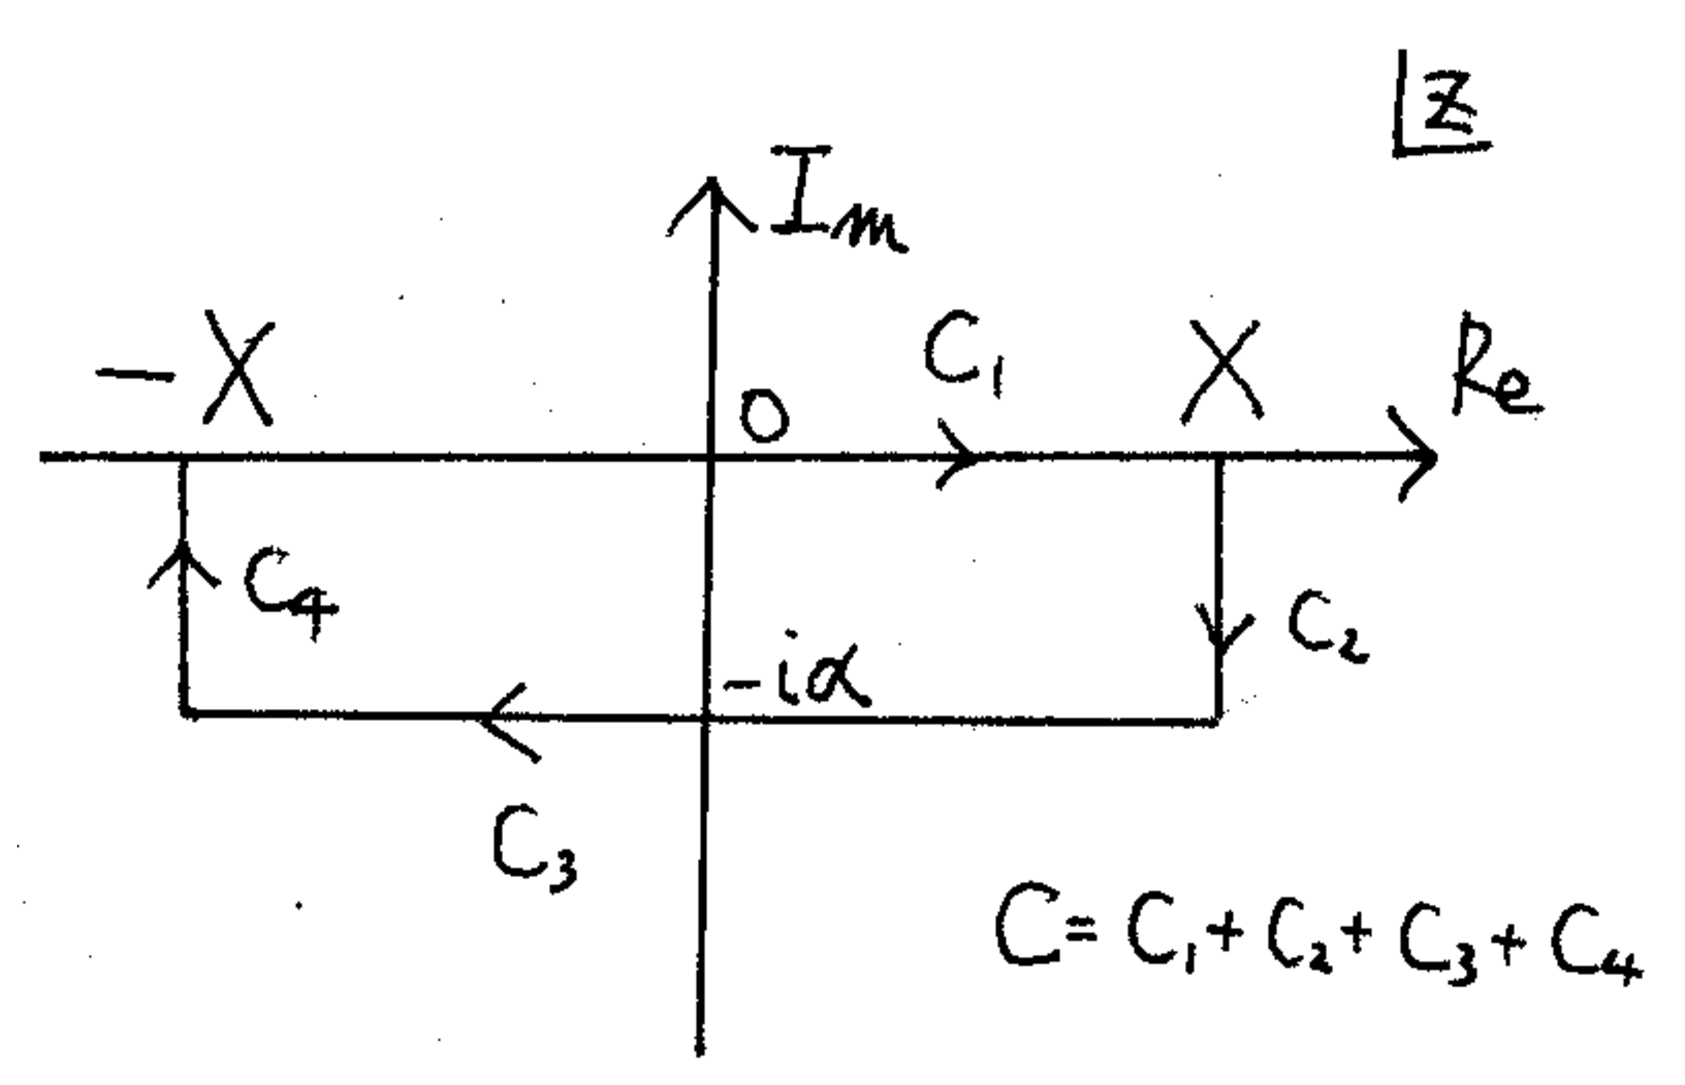
\includegraphics[width=0.4\hsize,clip]{2003math2-1.eps}
 \end{center}
 \caption{3.(別解)における積分経路}
 \ilabel{2003math2-1}
\end{figure}%

まず、$\mathrm{e}^{-az^2}$は至るところ正則だから、
Cauchyの積分定理より
\begin{eqnarray}
 \oint_C \mathrm{e}^{-a z^2} \mathrm{d} z = 0.  \ilabel{eq:a3}
\end{eqnarray}
一方、積分経路を$C=C_1+C_2+C_3+C_4$と分解し、
その各々について$X \to \infty$における積分を評価すると
\begin{eqnarray}
 && \int_{C_1} \mathrm{e}^{-az^2} \mathrm{d} z = \int_{-X}^X \mathrm{e}^{-ax^2} \mathrm{d} x \to \int_{-\infty}^\infty \mathrm{e}^{-ax^2} \mathrm{d} x
  \notag \\
 && \int_{C_3} \mathrm{e}^{-az^2} \mathrm{d} z = \int_X^{-X} \mathrm{e}^{-a(x-\mathrm{i}\alpha)^2} \mathrm{d} x = -\int_{-X}^X \mathrm{e}^{-a(x-\mathrm{i}\alpha)^2} \mathrm{d} x \to -\int_{-\infty}^\infty \mathrm{e}^{-a(x-\mathrm{i}\alpha)^2} \mathrm{d} x  \notag \\
 && \left| \int_{C_2} \mathrm{e}^{-az^2} \mathrm{d} z \right| \leq \max_{z \in C_2} \left| \mathrm{e}^{-az^2} \right| \cdot \int_{C_2} \left| \mathrm{d} z \right| = \mathrm{e}^{-a(X^2 - \alpha^2)} \cdot \alpha \to 0  \notag \\
 && \left| \int_{C_4} \mathrm{e}^{-az^2} \mathrm{d} z \right| \leq \max_{z \in C_4} \left| \mathrm{e}^{-az^2} \right| \cdot \int_{C_4} \left| \mathrm{d} z \right| = \mathrm{e}^{-a(X^2 - \alpha^2)} \cdot \alpha \to 0  \notag
\end{eqnarray}
となる。
従って、$X \to \infty$で
\begin{eqnarray}
 \oint_C \mathrm{e}^{-az^2} \mathrm{d} z
 \to \int_{-\infty}^\infty \mathrm{e}^{-ax^2} \mathrm{d} x - \int_{-\infty}^\infty \mathrm{e}^{-a(x-\mathrm{i}\alpha)^2} \mathrm{d} x  \ilabel{eq:a4}
\end{eqnarray}
が成り立つ。

以上、(\iref{eq:a3})(\iref{eq:a4})とGauss積分の公式から
\begin{eqnarray}
 \int_{-\infty}^\infty \mathrm{e}^{-a(x-\mathrm{i}\alpha)^2} \mathrm{d} x
 = \int_{-\infty}^\infty \mathrm{e}^{-ax^2} \mathrm{d} x = \sqrt{\frac{\pi}{a}}  \ilabel{eq:a6}
\end{eqnarray}
が成立する。これと(\iref{eq:a1})より
\begin{eqnarray}
 \int_{-\infty}^\infty \mathrm{e}^{-ax^2 + \mathrm{i} bx} \mathrm{d} x = \mathrm{e}^{-\frac{b^2}{4a}} \sqrt{\frac{\pi}{a}}  \ilabel{eq:a7}
\end{eqnarray}
であるから、求めるべき積分は
\begin{eqnarray}
 \int_{-\infty}^\infty \mathrm{e}^{\mathrm{i} ky} \mathrm{e}^{-a^2 k^2 t} \mathrm{d} k
 = \frac{1}{a} \sqrt{\frac{\pi}{t}} \exp \left( -\frac{y^2}{4a^2 t} \right)
  \ilabel{eq:a8}
\end{eqnarray}
である。

\item

(\iref{eq:3})(\iref{eq:5})より
\begin{eqnarray}
 u(x,t)
 &=& \frac{1}{2\pi} \int_{-\infty}^\infty \mathrm{d} k \int_{-\infty}^\infty \mathrm{d} \pr{x}
    f(\pr{x}) \mathrm{e}^{-\mathrm{i} k\pr{x}} \mathrm{e}^{\mathrm{i} kx +\mathrm{i}\omega t}  \notag \\
 &=& \frac{1}{2\pi} \int_{-\infty}^\infty \mathrm{d} k \int_{-\infty}^\infty \mathrm{d} \pr{x}
    f(\pr{x}) \mathrm{e}^{\mathrm{i} k (x-\pr{x})} \mathrm{e}^{-a^2 k^2 t}  ~~~~(\because(\iref{eq:2}))
    \notag \\
 &=& \frac{1}{2\pi} \int_{-\infty}^\infty \mathrm{d} \pr{x} f(\pr{x}) \cdot
    \frac{1}{a} \sqrt{\frac{\pi}{t}}
    \exp \left[ -\frac{(x-\pr{x})^2}{4a^2 t} \right] ~~~~(\because(\iref{eq:8}))
    \notag \\
 &=& \frac{1}{2a\sqrt{\pi t}} \int_{-\infty}^\infty \mathrm{d} \pr{x} f(\pr{x})
    \exp \left[ -\frac{(x-\pr{x})^2}{4a^2 t} \right]  \ilabel{eq:9}
\end{eqnarray}
と求まる。

\item

題意より
\begin{eqnarray}
 u(x,t)
 &=& \frac{U}{2a\sqrt{\pi t}} \int_{-L}^L \mathrm{d} \pr{x}
    \exp \left[ -\frac{(x-\pr{x})^2}{4a^2 t} \right]  \notag \\
 &=& \frac{U}{2a\sqrt{\pi t}} \cdot 2a\sqrt{t}
    \int_\frac{-x-L}{2a\sqrt{t}}^\frac{-x+L}{2a\sqrt{t}} \mathrm{e}^{-y^2} \mathrm{d} y
    ~~~~\left( y \equiv \frac{\pr{x}-x}{2a\sqrt{t}} \right) \notag \\
 &=& \frac{U}{2} \left[ \erf \left( \frac{-x+L}{2a\sqrt{t}} \right) 
    -\erf \left( \frac{-x-L}{2a\sqrt{t}} \right) \right]  \ilabel{eq:10}
\end{eqnarray}
と表される。
\end{enumerate}
\end{answer}


\end{document}
